\documentclass[11pt]{article}

\usepackage[letterpaper,margin=0.75in]{geometry}
\usepackage{booktabs}
\usepackage{graphicx}
\usepackage{listings}
\usepackage{mathtools}
\usepackage{underscore}

\setlength{\parindent}{1.4em}

\begin{document}

\lstset{
  language=Python,
  basicstyle=\small,          % print whole listing small
  keywordstyle=\bfseries,
  identifierstyle=,           % nothing happens
  commentstyle=,              % white comments
  stringstyle=\ttfamily,      % typewriter type for strings
  showstringspaces=false,     % no special string spaces
  numbers=left,
  numberstyle=\tiny,
  numbersep=5pt,
  frame=tb,
}

\title{Lab 2 Report}

\author{Nathan Davis}

\date{Feb 20, 2016}

\maketitle

\section{Reliable Transport}

\subsection{Network Setup}

For the networks in this paper, we set up two nodes. We used the same structure for each part and varied the queue length and loss rates. The configuration looks like this:

\vspace{5mm}

\begin{lstlisting}
    # n1 -- n2
    #
    n1 n2
    n2 n1

    # link configuration
    n1 n2 1Mbps 1000ms
    n2 n1 1Mbps 1000ms
\end{lstlisting}

\vspace{5mm}

\subsection{Sender Side TCP Implementation}

We used the transfer.py file from bene/examples as a base point to test my tcp implementation.

Beginning with the send method of TCP we put all the data it received into the send buffer.

\vspace{5mm}

\begin{lstlisting}
    def send(self,data):
        ''' Send data on the connection. Called by the application. This
            code uses the SendBuffer to send incrementally '''
        self.send_buffer.put(data)
        self.queue_packets()
\end{lstlisting}

\vspace{5mm}

We created a custom method called queue_packets, used only internally, that sends as many packets as possible, given the constraints of data availability and window size.

\vspace{5mm}

\begin{lstlisting}
    def queue_packets(self):
        ''' Send the next set of packets if there's any to send. Limit based
            on window size and the number of outstanding packets '''
        while True:
            if self.send_buffer.available() <= 0:
                break
            if self.send_buffer.outstanding() + self.mss > self.window:
                break
            packet_data = self.send_buffer.get(self.mss)
            self.send_packet(packet_data[0], packet_data[1])
\end{lstlisting}

\vspace{5mm}

The queue_packets method relies on the send_packet method given in the original TCP implementation. We did not change that method at all. However, it must be noted that the send_packet method sets a timer for the first packet it receives. This timer triggers a retransmission after the alloted timeout. We'll discuss later how that timeout is determined.

\vspace{5mm}

The retransmission method gets the next data to send, based on what's been ACKed, and sends that in a packet. We set the timeout to double so that it won't cause network congestion if there's major loss somewhere along the line. We also set another timeout in case this retransmission is lost.

\vspace{5mm}

\begin{lstlisting}
    def retransmit(self,event):
        ''' Retransmit data. '''
        self.trace("%s (%d) retransmission timer fired" % (self.node.hostname,self.source_address))
        packet_data = self.send_buffer.resend(self.mss)
        self.send_packet(packet_data[0], packet_data[1])
        self.timeout = self.timeout * 2
        self.trace("doubled the timeout to %f" % self.timeout)
        self.timer = Sim.scheduler.add(delay=self.timeout, event='retransmit', handler=self.retransmit)
\end{lstlisting}

\vspace{5mm}

We expect the receiver to send ACKs and we handle those using the method below. We use the slide method on the send_buffer to mark that data as "received" and we send the next set of packets using the queue_packets method. We also set the sequence so that we can keep track of what the receiver has confirmed.

\vspace{5mm}

The handle_ack method also handles RTT calculations which we'll discuss later.

\vspace{5mm}

\begin{lstlisting}
    def handle_ack(self,packet):
        ''' Handle an incoming ACK. '''
        ...
        self.sequence = packet.ack_number
        self.send_buffer.slide(packet.ack_number)
        self.cancel_timer()
        if self.send_buffer.outstanding() or self.send_buffer.available():
            self.timer = Sim.scheduler.add(delay=self.timeout, event='retransmit', handler=self.retransmit)
            self.queue_packets()
\end{lstlisting}

\vspace{5mm}

\subsection{Receiver Side TCP Implementation}

The receiver uses the ReceiveBuffer to keep track of data in order. When it receives a packet, it puts the packet in the receive buffer and sends an ACK for that data. It also delivers any data that's ready to the application.

\vspace{5mm}

\begin{lstlisting}
    def handle_data(self,packet):
        ''' Handle incoming data. This code currently gives all data to
            the application, regardless of whether it is in order, and sends
            an ACK.'''
        self.trace("%s (%d) received TCP segment from %d for %d" % (self.node.hostname,packet.destination_address,packet.source_address,packet.sequence))
        self.receive_buffer.put(packet.body, packet.sequence)
        data = self.receive_buffer.get()
        self.ack = len(data[0]) + data[1]
        self.app.receive_data(data[0])
        self.send_ack(packet.sent_time)
\end{lstlisting}

\vspace{5mm}

The method that sends an ACK is a simple packet with the ACK attribute set.

\vspace{5mm}

\begin{lstlisting}
    def send_ack(self, packet_sent_time=0):
        ''' Send an ack. '''
        packet = TCPPacket(source_address=self.source_address,
                           source_port=self.source_port,
                           destination_address=self.destination_address,
                           destination_port=self.destination_port,
                           sequence=self.sequence,ack_number=self.ack,
                           sent_time=packet_sent_time)
        # send the packet
        self.trace("%s (%d) sending TCP ACK to %d for %d" % (self.node.hostname,self.source_address,self.destination_address,packet.ack_number))
        self.transport.send_packet(packet)
\end{lstlisting}

\vspace{5mm}

\subsection{Timing Calculations}

These calculations are implemented inside the handle_ack method.

\vspace{5mm}

Whenever a packet is sent from the sender side, it's given a timestamp. That timestamp is transferred to the ACK on the receiver side and sent back. By comparing that timestamp to the current time, we can get a sample RTT.

\vspace{5mm}

\begin{lstlisting}
    # Calculate Sample RTT
    sample_rtt = Sim.scheduler.current_time() - packet.sent_time
    self.trace("sample round trip time %f" % sample_rtt)
\end{lstlisting}

\vspace{5mm}

We used the sample RTT to calculate the estimated RTT. If the estimated RTT has not been set yet, we set the estimated RTT to the sample RTT.

\vspace{5mm}

The calculation uses exponential backoff to place a heavier weight on more recent samples. The way it is calculated, it takes a percentage of its current value and adds in the new average from the sample RTT. This means that over time, samples that were taken earlier are given less weight than samples taken more recently.

\vspace{5mm}

The calculation uses alpha as the control for how much each portion should be weighted.

\vspace{5mm}

\begin{lstlisting}
    # Calculate the new estimated RTT
    alpha = 0.125
    if not self.estimated_rtt:
        self.estimated_rtt = sample_rtt
    else:
        self.estimated_rtt = (1 - alpha) * self.estimated_rtt + alpha * sample_rtt
\end{lstlisting}

\vspace{5mm}

Then we use the sample RTT and the estimated RTT to calculate a deviation. If the deviation has not been set yet, we initialize it to half of the estimated RTT.

\vspace{5mm}

\begin{lstlisting}
    # Calculate the deviation of the sample RTT
    beta = 0.25
    if not self.deviation_rtt:
        self.deviation_rtt = self.estimated_rtt/2
    else:
        self.deviation_rtt = (1 - beta) * self.deviation_rtt + beta * abs(sample_rtt - self.estimated_rtt)
\end{lstlisting}

\vspace{5mm}

Finally, we use that deviation of the RTT to calculate the timeout. That timeout is used when setting a retransmission timeout. As the RTT increases, so does the timeout. This gives packets sufficient time to reach the destination and for an ACK to come back and helps to avoid overfrequent retransmissions.

\vspace{5mm}

\begin{lstlisting}
    # Calculate the Retransmission Timeout (RTO)
    self.timeout = self.estimated_rtt + 4 * self.deviation_rtt
    self.trace("changed the timeout to %f" % self.timeout)
\end{lstlisting}

\vspace{5mm}

\subsection{Testing}

For the testing we used the network described above. We set the window size to 3000 bytes and tested with loss rates of 0\%, 10\%, 20\%, and 50\%.

\vspace{5mm}

We run these using the following command. The -f flag specifies which file to send, the -w flag specifies how large the window should be, and the -l flag specifies the loss.

\vspace{5mm}

\begin{lstlisting}
    python transfer.py -f test.txt -w 3000 -l 0.0
\end{lstlisting}

\vspace{5mm}

The results for the test using 0\% loss were 

\vspace{5mm}

\begin{lstlisting}
    You imported the correct tcppacket
    You've imported the right tcp file
    0 n1 (1) sending TCP segment to 2 for 0
    0 n1 (1) sending TCP segment to 2 for 1000
    ...
    0.0732 n2 (2) sending TCP ACK to 1 for 10000
    0.0832 sample round trip time 0.020800
    0.0832 changed the timeout to 0.024803
    Total time: 0.083200 seconds

    File transfer correct!
\end{lstlisting}

\vspace{5mm}

Each time a packet successfully completes a trip, we see the output notifying us that a sample round trip time has been taken and that the timeout has changed. This shows us that the timeout is always slightly more than tha round trip time. In a real-world implementation we would constrain the timeout to a minimum of 1 second, however it's usefull to see that in certain circumstances, the timeout may be much smaller to improve performance.

\vspace{5mm}

The other tests had the following results. These show us that loss rate is not always determinate of speed. Notice how the test at 20\% loss was actually faster than the test at 10\%. Running these tests multiple times gave different speeds, with the exception of 0\% loss.

\vspace{5mm}

\begin{lstlisting}
    Loss Rate   Transmission Time
    0.00        0.083200 seconds
    0.10        0.142825 seconds
    0.20        0.085600 seconds
    0.50        240.983621 seconds
\end{lstlisting}

\vspace{5mm}

The trend is clear however that the higher the loss, the greater the time it takes to transmit in general.

\vspace{5mm}

Running these same tests on a slightly larger file with a larger window, we see the same trend.

\vspace{5mm}

\begin{lstlisting}
    python transfer.py -f internet-architecture.pdf -w 3000 -l 0.00
\end{lstlisting}

\vspace{5mm}

\begin{lstlisting}
    Loss Rate   Transmission Time
    0.00        3.578016 seconds
    0.10        7.461133 seconds
    0.20        10.506584 seconds
    0.50        127486.273711 seconds
\end{lstlisting}

\vspace{5mm}

\section{Experiments}

\subsection{Changing Window Size}

For this portion, we sent the larger test file usind different window sizes. The loss rate was kept constant at 0\% and we look at  the throughput and an average of the queuing delay.

\vspace{5mm}

We used the command line to run the expirement with different window sizes. The -f flag was used to designate a large pdf file. The -q flag was used to toggle into the network with a queue limit of 100. The -l flag is used to ensure the loss is 0\% and the -w flag is used to change the window sizes. We used window sizes of 1000, 2000, 5000, 10000, 15000, and 20000.

\vspace{5mm}

\begin{lstlisting}
    python transfer.py -f internet-architecture.pdf -q -l 0.0 -w 1000
\end{lstlisting}

\clearpage
\subsection{Overall Time}

The first thing we observed is that the experiments with larger window sizes had a much smaller overall transmission time than those with smaller window sizes. The graph below illustrates how the total time decreases quickly in the beginning and then levels off as it approaches zero.

\vspace{5mm}

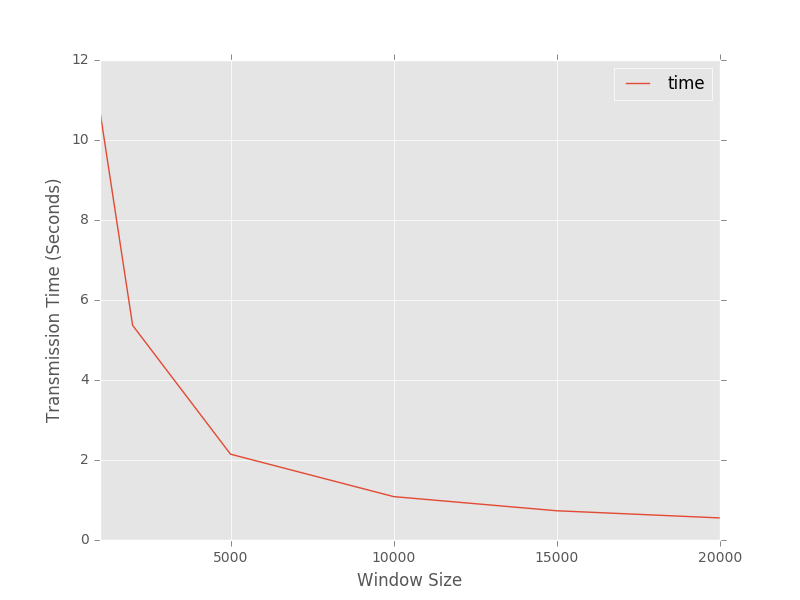
\includegraphics[width=17cm]{graphs/time-graph.png}

\clearpage
\subsection{Average Queueuing Delay}

The average queueing delay increased exponentially as the window size increased. This is because the sending side puts as many things in the queue as possible. Some of the packets may have even been dropped due to the lack of space in the queue. That queueing delay wouldn't even be accounted for in the graph below.

\vspace{5mm}

The graph below represents an average queueing delay for all the packets that were received by the receiver. It does not take into account the queueing delay for ACKs or lost packets.

\vspace{5mm}

Because the queuing delay increases exponentially, we could expect it to offset the window at some point and cause the overall time to increase. We would definitely expect to see higher values if more than one connection was running at a time. In a real network, multiple machines are sending and receiving and so routers can become congested. However, in this simulation we have only one bi-directional connection.

\vspace{5mm}

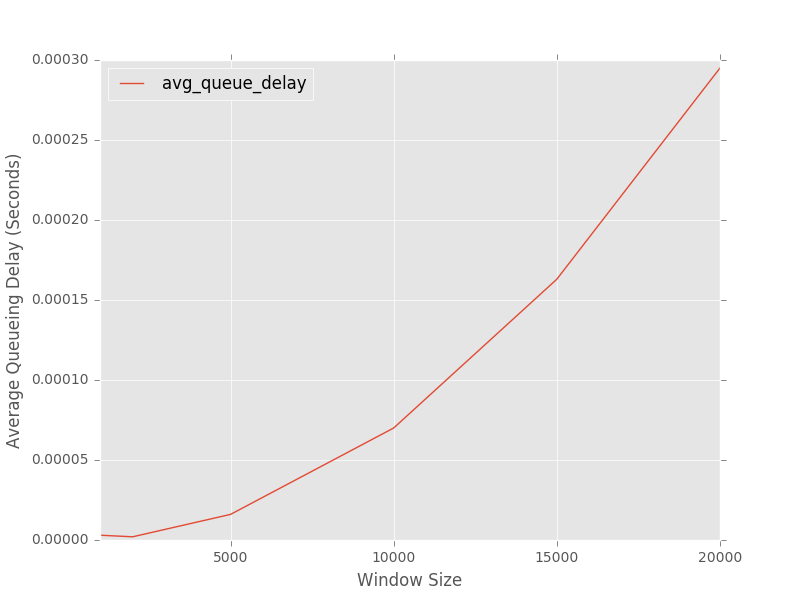
\includegraphics[width=17cm]{graphs/avg-queue-graph.png}

\clearpage
\subsection{Max Queueuing Delay}

Another measure we found interesting was the max queueing delay. This shows a linear increase and is most likely caused by the first set of packets sent. They would all be placed in the send queue at once and so the last of those packets would be likely to have the maximum queueing delay.

\vspace{5mm}

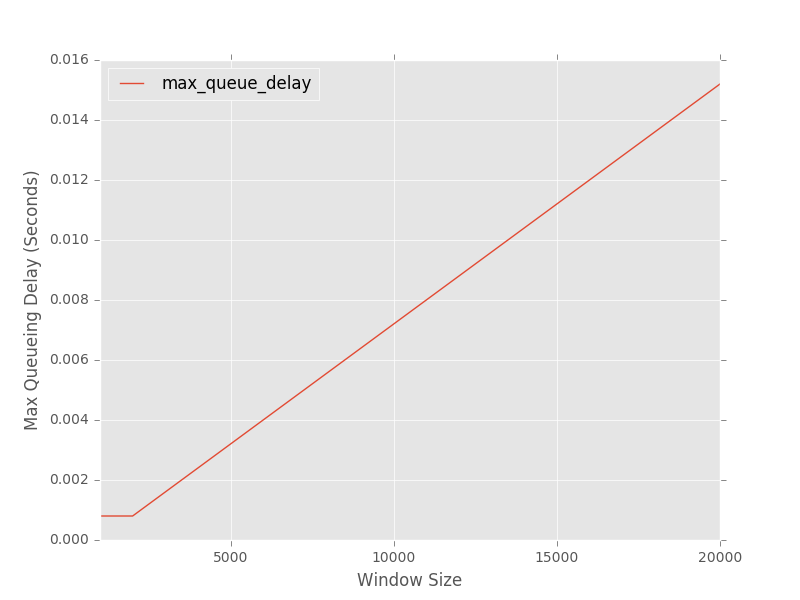
\includegraphics[width=17cm]{graphs/max-queue-graph.png}

\clearpage
\subsection{Throughput}

Finally, the throughput shows a linear increase. In general, this would point to a trend that larger window sizes tend to be faster. The fact that the throughput growth appears to be lindear was a little surprising as the size of the file is the same for every run and the time is shown to decrease rapidly at first and then taper off. We expected the throughput to increase rapidly at first and then taper off as it approaches a maximum.

\vspace{5mm}

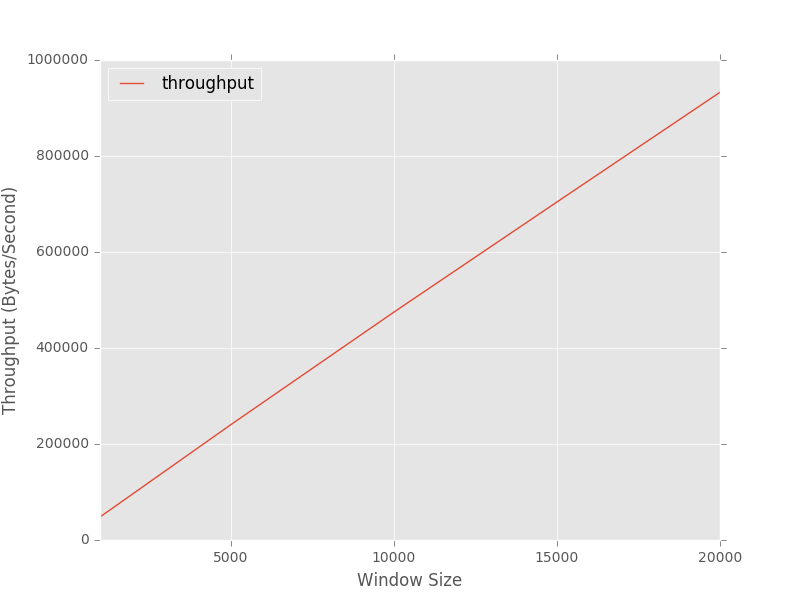
\includegraphics[width=17cm]{graphs/throughput.png}

\vspace{5mm}

\end{document}
